\subsubsection{Klausur}
Wie in Abbildung \ref{fig:klausur_reliability_score} zu sehen ist, blieb der Score bei den Klausuren unter Average Load bei jedem Testdurchlauf unter 20 von 100 Punkten.
Im zweiten Testdurchlauf gab es einen Ausschlag der k3s-Umgebung, in der ein Score von 0 Punkten erreicht wurde.
In den übrigen Testdurchläufen konnte die k3s-Umgebung einen besseren Score erzielen, blieb aber jedes Mal unter dem Score der Docker-Compose-Umgebung.
Dabei kann in Tabelle \ref{tab:klausur_average_load_metrics} erneut eine hohe Fehlerrate festgestellt werden, wobei diese in der Docker-Compose-Umgebung mehr als die Hälfte kleiner ist als in der k3s-Umgebung.
Die Anwendung in der Docker-Compose-Umgebung verbraucht aber wieder deutlich mehr CPU als in der k3s-Umgebung.
Auffällig ist auch, dass die k3s-Umgebung achtmal Pods neustarten musste.

\begin{table}[htbp]
\centering
\caption{Vergleich der Durchschnittswerte aller Test zur bestimmung der Zuverlässigkeit für das Klausur-Szenario unter Average Load}
\label{tab:klausur_average_load_metrics}

\begin{tabular}{lrr}
\toprule
\textbf{Metrik} & \textbf{Docker} & \textbf{K3s} \\
\midrule
Error Rate [\%]        & 5.43 & 12.05 \\
CPU Max [\%]           & 99.64 & 27.91 \\
Memory Max [\%]        & 63.12 & 19.80 \\
Node CPU Max [\%]      & 99.67 & 101.98 \\
Node Memory Max [\%]   & 66.95 & 78.60 \\
Restarts               & 0.00 & 8.00 \\
\bottomrule
\end{tabular}

\end{table}

\begin{figure}[htbp]
\centering
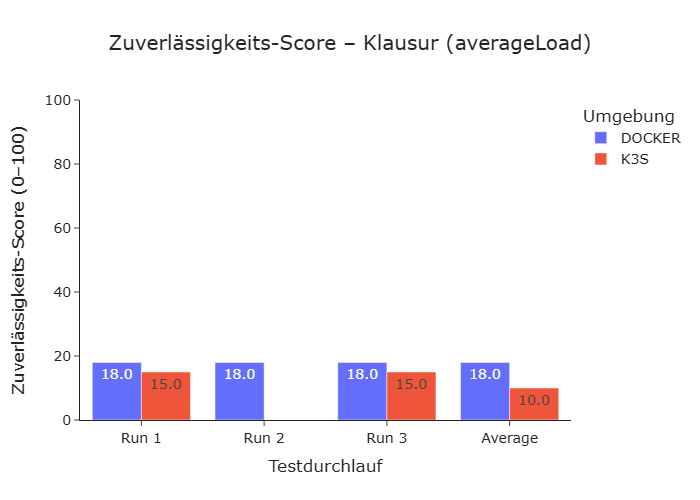
\includegraphics[width=0.8\textwidth]{bilder/tests/reliability_score_klausur_averageLoad.png}
\caption{Reliability Score für das Klausur-Szenario unter Average Load}
\label{fig:klausur_reliability_score}
\end{figure}

Beim Vergleich der durchschnittlichen Zuverlässigkeitswerte jeder Testmethode im Szenario „Klausur“, die in der Tabelle \ref{tab:scenario_score_matrix_klausur} zu sehen ist, fällt auf, dass die Docker-Compose-Umgebung wieder fast immer einen höheren Score als die k3s-Umgebung erzielt hat, bis auf den Spike-Test.
Dennoch bleibt festzuhalten, dass sich die Umgebungen nicht zu stark unterscheiden.
\begin{table}[htbp]
\centering
\caption{Durchschnittlicher Reliability Score pro Testtyp für das Szenario Klausur}
\label{tab:scenario_score_matrix_klausur}

\begin{tabular}{lccccc}
\toprule
\textbf{Environment} & \textbf{Smoke} & \textbf{Average Load} & \textbf{Stress} & \textbf{Spike} & \textbf{Breaking Point} \\
\midrule
Docker & 55.00 & 18.00 & 18.00 & 18.00 & 18.00 \\
K3s    & 41.33 & 10.00 & 17.00 & 23.00 & 6.67 \\
\bottomrule
\end{tabular}

\end{table}
\FloatBarrier